\documentclass{article}
\usepackage[utf8]{inputenc}
\usepackage[english]{babel}
\usepackage{lipsum,lineno}
\usepackage{amsmath}
\usepackage{amssymb}
\usepackage{mathtools}
\usepackage{tikz}
\usepackage{graphicx}
\usepackage{textcomp}
\usepackage{enumerate}
\usepackage{float}
\graphicspath{./images/}
\usepackage[dvipsnames]{xcolor}

\DeclareRobustCommand{\qdist}[1]{\ifmmode\langle#1\rangle\else\textlangle#1\textrangle\fi}


\DeclarePairedDelimiterX{\infdivx}[2]{(}{)}{%
  #1\;\delimsize\|\;#2%
}
\newcommand{\infdiv}{D\infdivx}
\DeclarePairedDelimiter{\norm}{\lVert}{\rVert}

\newcommand*\circled[1]{\tikz[baseline=(char.base)]{%
            \node[shape=circle,fill=blue!20,draw,inner sep=2pt] (char) {#1};}}

\usepackage{enumitem}

\usepackage[ 
  paperwidth = 168.3mm,
  paperheight = 260.4mm,
  top = 6mm,
  bottom = 7mm,
  outer = 6mm,
  inner = 20mm
]{geometry}

\setlength\parindent{0pt}

\newcommand{\CommentFontSize}{21}
\newcommand{\CommentSkipMult}{25}

\newcommand{\UserFontSize}{16}
\newcommand{\UserSkipMult}{0}

\newcommand{\DateFontSize}{15}
\newcommand{\DateSkipMult}{0}



\newenvironment{commentTextFont}
 {\fontfamily{mdugm}%
  \fontsize{\CommentFontSize}{\CommentSkipMult}%
  \selectfont}
 {\par}

 \newenvironment{userFont}
 {\fontfamily{mdugm}%
  \fontsize{\UserFontSize}{\UserSkipMult}%
  \selectfont}
 {\par}

 \newenvironment{dateFont}
 {\fontfamily{mdugm}%
  \fontsize{\DateFontSize}{\DateSkipMult}%
  \selectfont}
 {\par}

 \newcommand{\uComment}[3]{%
  \filbreak
  \begin{commentTextFont}#1\end{commentTextFont}%
  \vspace*{0.5cm}
  \begin{userFont}\textit{#2}\hspace*{\fill}%
  \begin{dateFont}#3\end{dateFont}\end{userFont}%
  \vspace*{0.8cm}
}

\newcommand{\nobarfrac}{\genfrac{}{}{0pt}{}}

\newcommand{\numberset}[1]{\mathbb{#1}}
\newcommand{\nat}{\numberset{N}}

\DeclarePairedDelimiter\abs{\lvert}{\rvert}%


\makeatletter
\let\oldabs\abs
\def\abs{\@ifstar{\oldabs}{\oldabs*}}
%
\let\oldnorm\norm
\def\norm{\@ifstar{\oldnorm}{\oldnorm*}}
\makeatother

\author{}

\begin{document}



\raggedright



\title{Advanced Engineering Mathematics}

\date{\vspace{-5ex}}

\maketitle

\section{SERIES}
\indent A \underline{sequence} is a list of terms that have been arranged in a certain order.\medskip

\noindent A \underline{series} is the sum of all the terms in a sequence. However, there has to be a definite relationship
between all the terms.
\subsection{ARITHMETIC SEQUENCE}


A \underline{sequence} is \underline{arithmetic} if \({d} \in \mathbb{R} \ni \forall {k} \in \mathbb{Z}^{+} \), 
\[a_{k+1} = a_{k+d}\]
where \(d = a_{k+1} - a_k\) is the common difference

\noindent and \(d = a_k + (n-k)d\) is the nth term of the sequence\medskip


\noindent \underline{NOTATION}:
 $ \{ a_n \} $ or $ \{ a_n \}_{n=1}^{\infty}$ 

\subsubsection{ARITHMETIC SERIES}
Partial Sum:

\[ S_n = \frac{n}{2}(2a_1 + (n-1)d)\]
Or
\[ S_n = \frac{n}{2}(a_1 + a_n)\]

\subsection{GEOMETRIC SEQUENCE}

A \underline{sequence} is \underline{geometric} if \(a_1 \ne 0 \) and if \( {r} \in \mathbb{R} \ne 0 \ni \forall k \in \mathbb{Z}\),

\[a_{k+1} = a_{k} r\]

\noindent where \(r = \frac{a_{k+1}}{a_k}\) is the common ratio\\
and \(a_n = a_k r^{n-k}\) is the nth term

\subsubsection{GEOMETRIC SERIES}

 \[ \sum_{n=1}^{\infty} a^{n-1} = {a + ar + ar^{2} + ...} \]

\noindent is convergent if \(\abs{r} < 1 \)\\
and the sum is 

\[ \sum_{n=1}^{\infty} ar^{n-1} = \frac{a}{1-r},  \abs{r} < 1\]

\subsection{CONVERGENCE}

A series \underline{converges} when the infinite sequence of the partial sums have a finite limit.\medskip

\noindent Any series in which individual terms approach zero \underline{converges.}\medskip

If $\sum_{n=1}^{\infty}a_n$ is \underline{convergent} then \( \lim_{n \to \infty} a_n = 0 \)

\subsection{DIVERGENCE}

A series \underline{diverges} when the infinite sequence of the partial sums does not have a finite limit.\medskip

\noindent Any series in which individual terms does not approach zero \underline{diverges}.

Given a series \( \ \sum_{n=1}^{\infty} a_n = a_1 + a_2 + a_3 + ...\),
\[S_n = \sum_{i = 1}^{n} a_i = a_1 + a_2 + ... + a_n\]

\noindent If $\{S_n\}$ is \underline{convergent} and \(\lim_{n \to \infty} S_n = s\) exists as a real number, then \( \sum a_n\) is called
\underline{convergent} and 

\[a_1 + a_2 + .... + a_n + ... = s\]

Or

\[\sum_{n=1}^{\infty} a_n = s\]

\noindent where s is the sum. Otherwise, the series is \underline{divergent}.

\subsection{TEST FOR DIVERGENCE}

If \( lim_{n \to \infty} a_n\) does not exist or
if \( lim_{n \to \infty} a_n \neq 0\), then the series \( \sum_{n=1}^{\infty} a_n\) is \underline{divergent}.

\subsection{PROPERTIES OF CONVERGENT SERIES}

If \( \sum a_n \) and \( \sum b_n \) are \underline{convergent} series, then so are:

\begin{enumerate}[label=\protect\circled{\roman*}]
  \item \( \sum_{n=1}^{\infty} ca_n = c \sum_{n=1}^{\infty} a_n\)
  \item \( \sum_{n=1}^{\infty} ( a_n + b_n ) = \sum_{n=1}^{\infty} a_n + \sum_{n=1}^{\infty} b_n\)
  \item \( \sum_{n=1}^{\infty} ( a_n - b_n ) = \sum_{n=1}^{\infty} a_n - \sum_{n=1}^{\infty} b_n\)
\end{enumerate}

\subsection{INTEGRAL TEST}

Suppose \(f\) is a \textit{continuous}, \textit{positive}, \textit{decreasing} function on \( [1,\infty)\).\\
\noindent Then \( \sum_{n=1}^{\infty} a_n \) is \underline{convergent} if and only if the improper integral \( \int_{1}^{\infty} f(x) dx \) is
convergent.

\begin{enumerate}[label=\protect\circled{\roman*}]
  \item If \( \int_{1}^{\infty} f(x) dx \) is \underline{convergent}, then \( \sum_{n=1}^{\infty} a_n\) is \underline{convergent}.
  \item If \( \int_{1}^{\infty} f(x) dx \) is \underline{divergent}, then \( \sum_{n=1}^{\infty} a_n\) is \underline{divergent}.
\end{enumerate}

\subsection{\(p\)-SERIES}

The \(p\)-series \( \sum_{n=1}^{\infty} \frac{1}{n^p} \) is \underline{convergent} if \( p > 1\) and \underline{divergent} if \( p \leq 1\).

\subsection{COMPARISON TEST}

Suppose \( \sum a_n \) and \( \sum b_n \) are series with \textit{positive} terms.

\begin{enumerate}[label=\protect\circled{\roman*}]
  \item If \( \sum b_n \) is \underline{convergent} and \( a_n \leq b_n \forall n \), then \( \sum a_n \) is \underline{convergent}. 
  \item If \( \sum b_n \) is \underline{divergent} and \( a_n \geq b_n \forall n \), then \( \sum a_n \) is \underline{divergent}.
\end{enumerate}

\subsection{LIMIT COMPARISON TEST}

Suppose \( \sum a_n\) and \( \sum b_n \) are series with \textit{positive} terms.

If \( \lim_{n \to \infty} \frac{a_n}{b_n} = c\)

where \(c\) is a finite number and \( c > 0 \), then both series either \underline{converge} or \underline{diverge}.\bigskip

\subsection{ALTERNATING SERIES TEST}

If the alternating series

\[ \sum_{n=1}^{\infty} (-1)^{n-1} b_n = b_1 - b_2 + b_3 - b_4 + b_5 - b_6 + ..., b_n > 0 \]

Satisfies 

\begin{enumerate}[label=\protect\circled{\roman*}]
  \item \( b_{n+1} \leq b_n \forall n \)
  \item \( \lim_{n \to \infty} b_n = 0\)
\end{enumerate}

then the series is \underline{convergent}.

\subsection{ABSOLUTE CONVERGENCE}

If \( \sum_{n=0}^{\infty} \abs{a_n}\) \underline{converges}, then \( \sum_{n=0}^{\infty} a_n\) \underline{converges}.

\subsection{CONDITIONAL CONVERGENCE}

If \( \sum a_n \) converges, but \( \abs{a_n} \) does not, \( \sum a_n \) \underline{converges conditionally}.

\subsection{RATIO TEST}

\begin{enumerate}[label=\protect\circled{\roman*}]
  \item If \( \lim_{n \to \infty} \abs{\frac{a_{n+1}}{a_n}} = L < 1\), then \( \sum_{n=1}^{\infty} a_n \) is \underline{absolutely convergent}.
  \item If \( \lim_{n \to \infty} \abs{\frac{a_{n+1}}{a_n}} = L > 1\) or \( \lim_{n \to \infty} \abs{\frac{a_{n+1}}{a_n}} = \infty \), then \( \sum_{n=1}^{\infty} a_n \) is \underline{divergent}.
  \item If \( \lim_{n \to \infty} \abs{\frac{a_{n+1}}{a_n}} = 1\), then the test is \underline{inconclusive}*.
\end{enumerate}

*use another test.

\subsection{ROOT TEST}

\begin{enumerate}[label=\protect\circled{\roman*}]
  \item If \( \lim_{n \to \infty}\sqrt[n]{\abs{a_n}} = L < 1\), then \( \sum_{n=1}^{\infty} a_n \) is \underline{absolutely convergent}.
  \item If \( \lim_{n \to \infty}\sqrt[n]{\abs{a_n}} = L > 1\) or \( \lim_{n \to \infty}\sqrt[n]{\abs{a_n}} = \infty\), then \( \sum_{n=1}^{\infty} a_n \) is \underline{divergent}.
  \item If \( \lim_{n \to \infty}\sqrt[n]{\abs{a_n}} = 1\), then the test is \underline{inconclusive}*.
\end{enumerate}

*use another test.

\subsection{POWER SERIES}

A power series is a series of the form

\[ \sum_{n=0}^{\infty} c_n x^n = c_0 + c_1 x + c_2 x^2 + c_3 x^3 + ...\]

where \(x\) is a variable and the \( c_n \)'s are the coefficients of the series.

A power series may \underline{converge} for some values of \(x\) and \underline{diverge} for other values of \(x\).
The sum of the series is a function

\[ f(x) = c_0 + c_1 x + c_2 x^2 + ... + c_n x^2 + ...\]

whose domain is the set of all \(x\) for which the series \underline{converges}.\bigskip

In general, a series of the form

\[ \sum_{n=0}^{\infty} c_n (x-a)^n = c_0 + c_1 (x-a) + c_2 (x-a)^2 + ...\]

is called a power series in \((x-a)\) or a power series centered at \(a\) or a power series
about \(a\).

\subsubsection{THEOREM}

For a given power series \( \sum_{n=0}^{\infty} c_n (x-a)^n \) there are only three possibilities:

\begin{enumerate}[label=\protect\circled{\roman*}]
  \item The series \underline{converges} only when \(x=a\)
  \item The series \underline{converges} \( \forall x \)
  \item There is a positive number \(R\) such that the series \underline{converges} if \( \abs{x-a} < R \) and \underline{diverges} if \( \abs{x-a} > R \).
\end{enumerate}

In general, the \underline{Ratio Test} (or sometimes the Root Test) should be used to determine the radius of convergence \( R \). The \underline{Root} and \underline{Ratio} Tests \textcolor{red}{\textit{always}} fail if \(x\) is an endpoint
of the interval of convergence, so the endpoints must be checked with some other test.

We can represent certain types of functions as sums of power series by manipulating geometric series or by differentiating such a series.
Expressing a known function as a sum of infinitely many terms is useful for integrating functions that don't have elementary
antiderivatives, for solving different equations, and approximating functions by polynomials.

Recall that:

\[ \frac{1}{1-x} = 1 + x + x^2 + x^3 + \dots = \sum_{n=0}^{\inf} x^n \qquad \abs{x} < 1 \]



\subsubsection{DIFFERENTIATION AND INTEGRATION OF POWER SERIES}

If the power series \( C_n(x-a)^n \) has radius of convergence \( R > 0 \) then the function \( f \) defined by

\[ f(x) = c_0 + c_1 (x-a) + c_2 (x-a)^2 + ... = \sum_{n=0}^{\infty} c_n (x-a)^n \]

is differentiable (and therefore continuous) on the interval \((a-R, a+R)\) and

\begin{enumerate}[label=\protect\circled{\roman*}]
  \item \( \frac{d}{dx} [\sum_{n=0}^{\infty} c_n (x-a)^n] = \sum_{n=0}^{\infty} \frac{d}{dx} [c_n (x-a)^n]\)
  \item \( \int [\sum_{n=0}^{\infty} c_n (x-a)^n] dx = \sum_{n=0}^{\infty} \int c_n (x-a)^n dx\)
\end{enumerate}

The radii of convergence of the power series in i and ii are both \( R \)

\subsection{TAYLOR SERIES}

If \( f \) has a power series representation (expansion) at \( a \), that is, if

\[ f(x) = \sum_{n=0}^{\infty} c_n (x-a)^n, \abs{x-a} < R\]

then its coefficients are given by the formula

\[ c_n = \frac{f^{(n)} (a)}{n!}\]

Substituting \( c_n \) back to the series gives

\[ f(x) = \sum_{n=0}^{\infty} \frac{f^{(n)} (a)}{n!} (x-a)^n\]

The above series is called the Taylor series of the function \( f \) at \( a \).

\subsection{MACLAURIN SERIES}

The special case \( a = 0\) of the Taylor series, such series becomes

\[ f(x) = \sum_{n=0}^{\infty} \frac{f^{(n)}(0)}{n!} x^n = f(0) + \frac{f'(0)}{1!} x + \frac{f''(0)}{2!} x^2 + \dots\]

This case arises frequently enough and is called the Maclaurin series.

\subsubsection{BINOMIAL SERIES}

If \(k \in \mathbb{R} \) and \( \abs{x} < 1 \), then

\[(1+x)^k = \sum_{n=0}^{\infty} (\nobarfrac{k}{n}) x^n = 1 + kx + \frac{k(k-1)}{2!} x^2 + \frac{k(k-1)(k-2)}{3!} x^3 + \dots \]

\subsubsection{MACLAURIN SERIES AND THEIR RADII OF CONVERGENCE}

\[ \frac{1}{1-x} = \sum_{n=0}^{\infty} x^n = 1 + x + x^2 + x^3 + \dots \qquad R = 1\] 
\[ e^x = \sum_{n=0}^{\infty} \frac{x^n}{n!} = 1 + \frac{x}{1!} + \frac{x^2}{2!} + \frac{x^3}{3!} + \dots \qquad R = \infty\]
\[ sinx = \sum_{n=0}^{\infty} (-1)^n \frac{x^{2n+1}}{(2n+1)!} = x - \frac{x^3}{3!} + \frac{x^5}{5!} - \frac{x^7}{7!} + \dots \qquad R = \infty \]
\[ cosx = \sum_{n=0}^{\infty} (-1)^n \frac{x^{2n}}{(2n)!} = 1 - \frac{x^2}{2!} + \frac{x^4}{4!} - \frac{x^6}{6!} + \dots \qquad R = \infty \]
\[ tan^{-1}x = \sum_{n=0}^{\infty} (-1)^n \frac{x^{2n+1}}{2n+1} = x - \frac{x^3}{3} + \frac{x^5}{5} - \frac{x^7}{7} + \dots \qquad R = 1 \]
\[ ln(1 + x) = \sum_{n=0}^{\infty} (-1)^{n-1} \frac{x^n}{n} = x - \frac{x^2}{2} + \frac{x^3}{3} - \frac{x^4}{4} + \dots \qquad R = 1 \]
\[ (1 + x)^k = \sum_{n=0}^{\infty} (\nobarfrac{k}{n}) x^n = 1 + kx + \frac{k(k - 1)}{2!} x^2 + \dots \qquad R = 1 \]

\section{SERIES SOLUTIONS OF LINEAR DIFFERENTIAL EQUATIONS}

\subsection{ANALYTIC AT A POINT}

A function \(f\) is analytic at a point \(a\) if it can be represented by a power series in \(x-a\) with a positive radius of convergence.\vspace{0.5cm}  

Examples:

\[e^x = 1 + \frac{x}{1!} + \frac{x^2}{2!} + \dots\]
\[sin x = x - \frac{x^3}{3!} + \frac{x^5}{5!} - \dots\]
\[cos x = 1 - \frac{x^2}{2!} + \frac{x^4}{4!} - \frac{x^6}{6!} + \dots\]\vspace{0.5cm}

for \(\abs{x} < \infty \). these Maclaurin series are analytic at \(x = 0\).

\subsection{SHIFTING THE SUMMATION INDEX}

Combining two or more summations as a single summation often requires reindexing, that is, a shift in the index of summation.\vspace{0.5cm}

\textbf{EXAMPLE}\vspace{0.5cm}

Write

\[\sum_{n=2}^{\infty}n(n-1)c_n x^{n-2} - \sum_{n=0}^{\infty} c_n x^{n+1}\]

As one power series.\vspace{0.5cm}

\textbf{SOLUTION}\vspace{0.5cm}

Write the first term of the first summation:\vspace{0.5cm}

at \(n = 2\):
\[\sum_{n=2}^{\infty}n(n-1)c_n x^{n-2} = (2)(2-1) c_2 x^{2-2}\]
the expression then becomes:
\[(2)(2-1) c_2 x^{2-2} + \sum_{n=3}^{\infty}n(n-1)c_n x^{n-2} - \sum_{n=0}^{\infty} c_n x^{n+1}\]
\[= 2c_2 + \sum_{n=3}^{\infty}n(n-1)c_n x^{n-2} - \sum_{n=0}^{\infty} c_n x^{n+1}\]
For the first summation, create a dummy variable \(k = n - 2\) and thus \(n = k + 2\). The first summation becomes:\vspace{0.5cm}
\[\sum_{k=1}^{\infty}(k+2)(k+1)c_{k+2} x^{k}\]
For the second summation, create a dummy variable \(k = n + 1\) and thus \(n = k - 1\). The second summation becomes:\vspace{0.5cm}
\[\sum_{k=1}^{\infty} c_{k-1} x^{k}\]

both summations now \textit{start at the same index} and have \textit{the same exponent of x}. You can now combine them:

\[2c_2 + \sum_{k=1}^{\infty}(k+2)(k+1)c_{k+2} x^{k} - \sum_{k=1}^{\infty} c_{k-1} x^{k}\]
\[= 2c_2 + \sum_{k=1}^{\infty}[(k+2)(k+1)c_{k+2}  - c_{k-1} ] x^{k}\]

\subsection{SOLUTIONS ABOUT ORDINARY POINTS}

Suppose the linear second order differential equation:

\[a_2(x)y'' + a_1(x)y' + a_0(x)y = 0\]\vspace{0.5cm}

divide by the leading coefficient \(a_2(x)\):
\[y'' + \frac{a_1(x)}{a_2(x)}y' + \frac{a_0(x)}{a_2(x)} y = 0\]

Let \(P(x) = \frac{a_1(x)}{a_2(x)}\) and \(Q(x) = \frac{a_0(x)}{a_2(x)}\); thus the standard form:

\[y'' + P(x)y' + Q(x)y = 0\]

\subsubsection{ORDINARY POINTS}

A point \(x_0\) is said to be the \textbf{ordinary point} of a differential equation if both \(P(x)\) and \(Q(x)\) are analytic at \(x_0\).
A point that is not an ordinary point is said to be a \textbf{singular point} of the equation. \vspace{0.5cm}

\textbf{Ordinary points} are extracted from the values of \(x\) in the expressions of the \underline{numerators}, while \textbf{singular points} can be extracted from
the expressions in the \underline{denominators}.


\subsubsection{POWER SERIES SOLUTIONS}

If \(x = x_0\) is an ordinary point of a differential equation, we can \textit{always find two linearly independent solutions} in the form of a power series centered at \(x_0\);\vspace{0.5cm}

that is,

\[y=\sum_{n=0}^{\infty} c_n (x-x_0)^n\]

A series solution converges at least on some interval defined by \( \abs{x-x_0} < R\), where \(R\) is the distance from \(x_0\) to the closest singular point.\vspace{0.5cm}

\textbf{Power series solutions} can only be used if a differential equation has an \textbf{ordinary point}.


\subsection{SOLUTIONS ABOUT SINGULAR POINTS}

A singular point is a \textbf{regular singular point} when the expression in the denominator of \(P(x)\) is \textit{at most} to the first degree and the expression in the denominator of 
\(Q(x)\) is \textit{at most} to the second degree. Otherwise, it is an \textbf{irregular singular point}.

\subsubsection{FROBENIUS METHOD}

If \(x = x_0\) is a regular point, then there exists at least one non-zero solution in the form

\[y = (x-x_0)^r \sum_{n=0}^{\infty} c_n (x-x_0)^n = \sum_{n=0}^{\infty} c_n(x-x_0)^{n+r}\]

where \(r\) is a constant to be determined. The series will converge at least on some given interval defined by \(0 < x - x_0 < R\).\\
Assume that \(c_0 \neq 0\).

\subsubsection{GENERAL INDICIAL EQUATION}

To determine the values of \(r_1\) and \(r_2\), we use the \textbf{general indicial equation} given by:

\[r(r-1) + a_0 r + b_0 = 0\] 
\[r^2 - r + a_0 r + b_0 = 0\]
rearranging,
\[r^2 + (a_0 - 1) r + b_0 = 0\]

which is in the form of a quadratic equation in standard form \(ar^2 + br + c = 0\), where \(a = 1\), \(b = a_0 - 1\) and \(c = b_0\).\vspace{0.5cm}

And thus the quadratic formula can be used to solve for \(r_1\) and \(r_2\):

\[r_{1,2} = \frac{-(a_0 - 1) \pm \sqrt{(a_0-1)^2 - 4(1)(b_0)}}{2(1)}\]

\subsubsection{CASE I}

If \(r_1\) and \(r_2\) are distinct (their difference is between 0 and 1), there exist two linearly independent solutions of the form

\[y_1(x) = \sum_{n=0}^{\infty} c_nx^{n+r_1}\]
\[y_2(x) = \sum_{n=0}^{\infty} b_nx^{n+r_2}\]

\subsubsection{CASE II}

If \(r_1 - r_2 = N\), where \(N\) is a positive integer, then there exist two linearly independent solutions of the form

\[y_1(x) = \sum_{n=0}^{\infty} c_nx^{n+r_1} \qquad ,c_0 \neq 0\]
\[y_2(x) = Cy_1(x)ln(x) + \sum_{n=0}^{\infty} b_nx^{n+r_2} \qquad ,b_0 \neq 0\]

Where C is a constant that could be zero.

\subsubsection{CASE III}

If r1 = r2, then there exist two linearly independent solutions of the form

\[y_1(x) = \sum_{n=0}^{\infty} c_nx^n+r_1 \qquad ,c_0 \neq 0\]
\[y_2(x) = y_1(x) ln(x) + \sum_{n=0}^{\infty} b_nx^{n+r_2}\]

if \(r_1 - r_2 = 0\), the method fails to give a series solution. However, if \(y_1(x)\) is a known solution, we can obtain the second solution using:

\[y_2(x) = y_1(x) \int \frac{e^{-\int P(x)dx}}{y_1^2(x)} dx\]

\section{Vector Analysis}

\subsection{Vectors in \(\mathbb{R}^{n}\)}
\subsubsection{Vectors in \(\mathbb{R}^{2}\)}

\textbf{Scalars vs Vectors:}\vspace{0.5cm}

\textbf{Scalar:} A quantity with a \textit{magnitude} (in simplest terms, just a number)\\
\textbf{Vector:} A quantity with both a \textit{magnitude} and \textit{direction} (weight, force)\vspace{0.5cm}

\subsubsection{Vector Notation and Terminology}

\(\overrightarrow{AB}\): a vector with start point at \(\mathbf{A}\) and terminal point at \(\mathbf{B}\)\\
\(\norm{\overrightarrow{\mathbf{AB}}}\): magnitude of a vector\\
\(\overrightarrow{AB} = \overrightarrow{CD}\): two vectors that have the same magnitude and direction\\
\(-\overrightarrow{AB}\): negative of a vector\\
\(k\overrightarrow{AB}\): scalar multiple of a vector\\
\(0\overrightarrow{AB} = 0\): the zero vector\vspace{0.5cm}

Vectors are \textit{free}— they can be moved to any new position if their magnitudes and directions are not changed.\vspace{0.5cm}

if \(k > 0\), \(k\overrightarrow{AB}\) has the same direction as \(\overrightarrow{AB}\)\\
if \(k < 0\), \(k\overrightarrow{AB}\) has the same direction, but opposite of \(\overrightarrow{AB}\)\\
Two vectors are \textit{parallel} if and only if they are nonzero scalar multiples of each other.\vspace{0.5cm}

\subsubsection{Vector Addition and Subtraction}

\begin{figure}[h]
  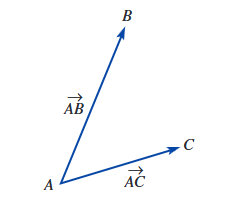
\includegraphics[width=5cm]{images/figure1.PNG}
  \centering
\end{figure}

If \(\overrightarrow{AB}\) and \(\overrightarrow{AC}\) are on the sides of a parallelogram, \(\overrightarrow{AD}\) is the sum of \(\overrightarrow{AB}\) and \(\overrightarrow{AC}\): 

\[\overrightarrow{AD} = \overrightarrow{AB} + \overrightarrow{AC}\]

\begin{figure}[h]
  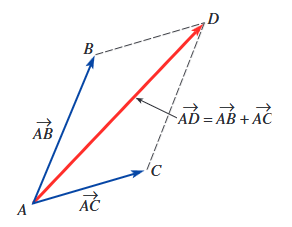
\includegraphics[width=5cm]{images/figure2.PNG}
  \centering
\end{figure}

The difference between two vectors:

\[\overrightarrow{AB} - \overrightarrow{AC} = \overrightarrow{AB} + (-\overrightarrow{AC})\]

\begin{figure}[h]
  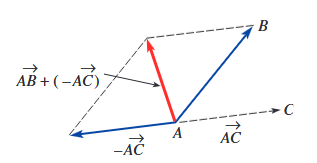
\includegraphics[width=5cm]{images/figure3.PNG}
  \centering
\end{figure}

The same vector difference can be interpretted as the third side of a triangle with sides \(\overrightarrow{AB}\) and \(\overrightarrow{AC}\):

\[\overrightarrow{CB} = \overrightarrow{AB} - \overrightarrow{AC}\]

\begin{figure}[h]
  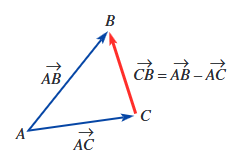
\includegraphics[width=5cm]{images/figure4.PNG}
  \centering
\end{figure}

\subsubsection{Vectors in a Coordinate Plane}

Suppose vectors are on a 2D plane.\\

A position vector of the point \(P\) is a vector with an initial point at origin \(O\) and a terminal point \(P(x_1 , y_1)\):

\[\overrightarrow{OP} = \qdist{x_1,y_1}\]

\begin{figure}[h]
  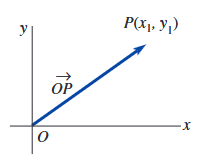
\includegraphics[width=5cm]{images/figure5.PNG}
  \centering
\end{figure}

\textbf{EXAMPLE 1}\\

The displacement from an initial point \(P_1(x,y)\) to a terminal point \(P_2(x + 4, y + 3)\)
is 4 units to the right and 3 units up.

\begin{figure}[h]
  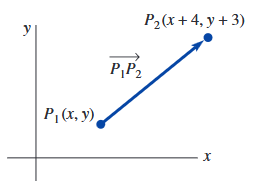
\includegraphics[width=5cm]{images/figure6.PNG}
  \centering
\end{figure}

The position vector \(a = \qdist{4,3}\) emanating from the origin is the equivalent to the displacement vector \(\overrightarrow{P_1 P_2}\) from \(P_1(x,y)\) to \(P_2(x+4,y+3)\).

\begin{figure}[H]
  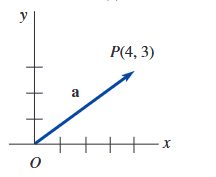
\includegraphics[width=5cm]{images/figure7.PNG}
  \centering
\end{figure}\vspace{0.5cm}

In general, a vector \(a\) in \(\mathbb{R}^{2}\) is any ordered pair of real numbers

\[a = \qdist{a_1, a_2}\]

The numbers \(a_1\) and \(a_2\) are components of vector \(a\).\vspace{0.5cm}

\textbf{Addition, Scalar Multiplication, Equality}\\
Let \(a = \qdist{a_1, a_2}\) and \(b = \qdist{b_1, b_2}\) be vectors in \(\mathbb{R}^{2}\).\\

\begin{enumerate}[label=\protect\circled{\roman*}]
  \item Addition: \(a + b = \qdist{a_1 + b_1, a_2 + b_2}\)
  \item Scalar Multiplication: \(ka = \qdist{ka_1, kb_1}\)
  \item Equality: \(a = b\) if and only if \(a_1 = b_1, a_2 = b_2\) 
\end{enumerate}

\textbf{Subtraction}\\

The \textit{negative} of a vector \textit{b} is defined by

\[-b = (-1)b = \qdist{-b_1,-b_2}\]

\textit{Subtraction} can then be defined by

\[a-b=a+(-b) = \qdist{a_1-b_1,a_2-b_2}\]

The sum of two vectors \(\overrightarrow{OP_1}\) and \(\overrightarrow{OP_2}\)

\begin{figure}[H]
  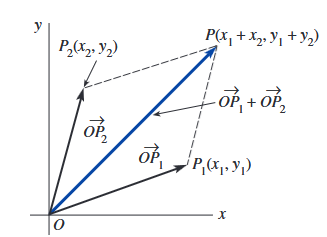
\includegraphics[width=6cm]{images/figure8.PNG}
  \centering
\end{figure}

The vector \(\overrightarrow{P_1 P_2}\) with initial point $P_1$ and terminal point $P_2$ is the difference of position vectors 

\[\overrightarrow{P_1 P_2} = \overrightarrow{OP_2} - \overrightarrow{OP_1} = \qdist{x_2 - x_1 , y_2 - Y_1}\]

\begin{figure}[H]
  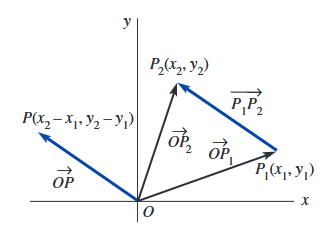
\includegraphics[width=8cm]{images/figure9.PNG}
  \centering
\end{figure}

The vector \(\overrightarrow{P_1 P_2}\) can be drawn either starting from the terminal point of \(OP_1\) to the terminal point of \(OP_2\), or as the position vector $\overrightarrow{OP}$ whose terminal point has coordinates $(x_2 - x_1, y_2 - y_1)$\vspace{0.5cm}

$\overrightarrow{OP}$ and $\overrightarrow{P_1 P_2}$ are considered equal, since the have the same magnitude and direction.\vspace{0.5cm}

\textbf{EXAMPLE 2}\\

if $a = \qdist{1,4}$ and $b = \qdist{-6,3}$, find:\\

\begin{itemize}
  \item $\mathbf{a+b}$\\
    $a + b =  \qdist{1 + (-6), 4 + 3} = \qdist{-5 , 7} $ 
  \item $\mathbf{a-b}$\\
    $a - b = \qdist{1 - (-6), 4 - 3} = \qdist{7 , 1}$
  \item $\mathbf{2a + 3b}$\\
    $2a + 3b = \qdist{2(1) + 3(-6),2(4) + 3(3)} = \qdist{2 + (-18), 8 + 9} = \qdist{-16,17} $
\end{itemize}

\textbf{Properties of Vectors}

\begin{enumerate}[label=(\roman*)]
  \item \textit{Commutative:} \(a + b = b+ a\)
  \item \textit{Associative:} \(a + (b + c) = (a + b) + c\)
  \item \textit{Additive Identity:} \(a + 0 = a\)
  \item \textit{Additive Inverse:} \(a + (-a) = 0\)
  \item \(k(a + b) = ka + kb\), $k$ a scalar
  \item \((k_1 + k_2)a = k_1 a + k_2 a\), $k_1$ and $k_2$ scalars
  \item \(k_1(k_2 a) = (k_1 k_2)a\), $k_1$ and $k_2$ scalars
  \item $1a = a$
  \item \textit{Zero Vector:} $0a = 0$ 
\end{enumerate}

the zero vector 0 in properties $(iii)$, $(iv)$, and $(ix)$ is defined as

\[0 = \qdist{0,0}\]

\textbf{Magnitude}\vspace{0.5cm}

The \textbf{magnitude}, \textbf{length} or \textbf{norm} of a vector $a$ is denoted by $\norm{a}$ \\
By pythagorean theorem,


\[\norm{a} = \sqrt{a^2 _1 + a ^2_2}\]

\(\norm{a} \geq 0 \) for any vector \(a\), and \(\norm{a} = 0\) if and only if \(a = 0\). For example, if \(a = \qdist{6,-2}\),

\[\norm{a} = \sqrt{6^2 + -2^2} = \sqrt{36 + 4} = \sqrt{40} = 2\sqrt{10}\]


\textbf{Unit Vectors}\vspace{0.5cm}

A vector of magnitude 1 is called a \textit{unit vector}.

\[\norm{u} = \norm{\frac{1}{\norm{a}} a} = \frac{1}{\norm{a}} \norm{a} = 1\]

write \(u = \frac{1}{\norm{a}} a\) as 

\[u = \frac{a}{\norm{a}}\]

\textbf{EXAMPLE 3}\vspace{0.5cm}

Given $\mathbf{a} = \qdist{2, -1}$, form a unit vector in the same direction as $\mathbf{a}$. In the opposited direction of $\mathbf{a}$.\vspace{0.5cm}

\textbf{SOLUTION}\vspace{0.5cm}

\[\norm{\mathbf{a}} = \sqrt{2^2 + (-1)^2} = \sqrt{5}\]

\[\mathbf{u} = \frac{1}{\sqrt{5}} \mathbf{a} = \frac{1}{\sqrt{5}} \qdist{2,-1} = \qdist{\frac{2}{\sqrt{5}},-\frac{1}{\sqrt{5}}}\]

In the opposite direction of $\mathbf{a}$:

\[\mathbf{-u} = \qdist{-\frac{2}{\sqrt{5}},\frac{1}{\sqrt{5}}}\]

If $\mathbf{a}$ and $\mathbf{b}$ are vectors and $c_1$ and $c_2$ are scalars, then $c_1 \mathbf{a} + c_2 \mathbf{b}$ is called a linear combination of $\mathbf{a}$ and $\mathbf{b}$.\vspace{0.5cm}

\textbf{The i, j Vectors}\vspace{0.5cm}

Any vector $\mathbf{a} = \qdist{a_1 , a_2}$ can be written as a sum:\\

\[\qdist{a_1,a_2} = \qdist{a_1,0} + \qdist{0,a_2} = a_1\qdist{1,0} + a_2\qdist{0,1}\]

The unit vectors $\qdist{a_1,a_2}$

\end{document}